\lab{Newton's Second Law}

\section*{Acceleration}

The acceleration of an object is a rate of change in its velocity:

\begin{eqnarray*}
	\mbox{acceleration} & = & \frac{\mbox{later velocity} - \mbox{earlier velocity}}{\mbox{time interval}} \\
	\vect{a} & = & \frac{\vectsub{v}{f} - \vectsub{v}{i}}{\Delta t} \\
	\vect{a} & = & \frac{\Delta \vec{v}}{\Delta t}
\end{eqnarray*}

Since velocity is a vector with both magnitude and direction, an object as non-zero acceleration if the (1) magnitude of velocity changes; (2) the direction of velocity changes; or (3) both magnitude and direction of velocity changes.

\subsection*{Speeding up and slowing down in a straight line}

If the magnitude of the velocity changes, but not its direction, then the object speeds up or slows down but continues to move in a straight line. An example is the fancart that you analyzed in a previous experiment. If the acceleration and velocity of the cart were in the same direction, then the cart sped up. If the acceleration and velocity of the cart were in opposite directions, then the cart slowed down. You can observe the fact that the cart is accelerating by viewing the marks. If the marks get further apart or closer together, then the object is accelerating.

\subsection*{Example}

\tightframe{

{\bf Question:}

Suppose that a puck starts at the right side and moves toward the left side of the image shown below. Marks show the position of the puck at equal time steps. Using our standard definitions of $+x$, $+y$, and $+z$ directions, what is the direction of the velocity and the acceleration of the puck? Is the puck speeding up or slowing down?

%\scaledimage{}{A puck at different instances of time.}{0.5}
\bigskip
\begin{center}
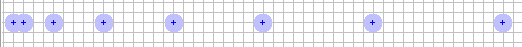
\includegraphics[scale=0.5]{newtons-second-law/puck}
\end{center}
\bigskip


{\bf Answer:}

The puck's velocity is in the direction it is moving which is to the left. Thus, its velocity is in the $-x$ direction. (You can say that its x-component is negative and its y and z components are zero.)

The puck is slowing down as observed by the decreasing distance between marks of the puck. Therefore, its acceleration is in the opposite direction as its velocity, or the $+x$ direction. 

}

\tightframe{

{\bf Question:}

Suppose that the puck in the previous question starts at the left side and moves toward the right side of the image. Marks show the position of the puck at equal time steps. Using our standard definitions of $+x$, $+y$, and $+z$ directions, what is the direction of the velocity and the acceleration of the puck? Is the puck speeding up or slowing down?

{\bf Answer:}

The puck's velocity is in the direction it is moving which is to the right. Thus, its velocity is in the $+x$ direction. (You can say that its x-component is negative and its y and z components are zero.)

The distance between marks of the puck is increasing; therefore, the puck is speeding up. As a result, its acceleration is in the same direction as the velocity (the $+x$ direction).

}

\bigskip
Note that the sign of the acceleration in both of the examples above is positive. It alone does not tell you whether the object will speed up or slow down.

\subsection*{Changing direction with constant speed}

Whenever an object travels along a curved path, it also has an acceleration. Even if it travels with a constant speed, the direction of its velocity changes; therefore, it has a non-zero acceleration.  We can calculate the acceleration in the same way: $\vect{a} = \frac{\Delta \vec{v}}{\Delta t}$. But to visualize the direction of the acceleration, you should find the direction of $\Delta \vec{v}$. Follow this procedure:

\begin{enumerate}
	\item Sketch the vectors $\vec{v}_f$ and $\vec{v}_i$.
	\item Off to the side, sketch $\vec{v}_f$ and $\vec{v}_i$ so that they are drawn tail to tail. Be sure to keep their lengths and directions the same.
	\item Sketch the vector $\Delta \vec{v}$ from the head of $\vec{v}_i$ to the head of $\vec{v}_f$
\end{enumerate}

For example, suppose an object travels in a circle with constant speed, as shown in Figure \ref{newtons-second-law/v-vectors}. Its velocity at two different instances of time is indicated. What is the direction of its acceleration during this time interval?

\scaledimage{newtons-second-law/v-vectors}{Velocity at two locations as it moves along a circle at constant speed.}{0.5}

If you draw the velocity vectors at any locations close together on the circle, you will find that the acceleration vector points toward the center. This is a general observation, \emph{the acceleration of an object that travels in a circle at a constant speed points toward the center of the circle.}

\subsection*{Example}

\tightframe{

{\bf Question:}

A puck bounces off the wall on an air hockey table as shown below. Draw the acceleration vector of the puck during the time interval of the collision.

\bigskip
\begin{center}
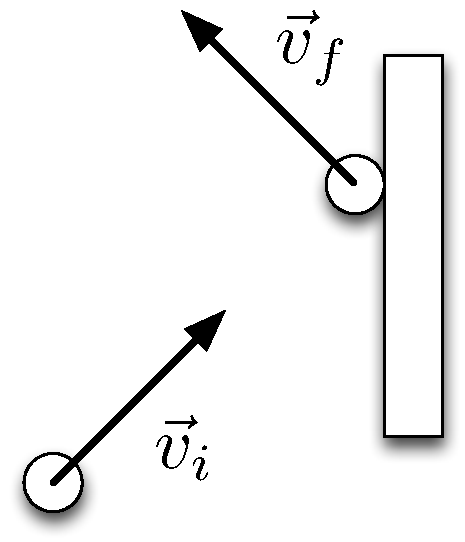
\includegraphics[scale=0.5]{newtons-second-law/wall}
\end{center}
\bigskip


{\bf Answer:}

Sketch the initial and final velocity vectors tail to tail. Then draw $\Delta \vec{v}$ from the head of $\vec{v}_i$ to the head of $\vec{v}_f$. This is the direction of the acceleration. In this case, you can see that it is perpendicular to the wall. The wall must be frictionless.

\bigskip
\begin{center}
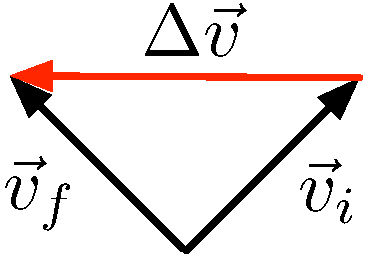
\includegraphics[scale=0.5]{newtons-second-law/collision-acc}
\end{center}
\bigskip

}

\section*{Newton's second law}

The sum of the forces acting on an object is called the \emph{net force}. A net force on an object causes it to accelerate. The object's acceleration is proportional to the net force on the object. The 

\begin{eqnarray*}
	\mbox{acceleration of an object} & = & \frac{\mbox{net force on the object}}{\mbox{mass of the object}} \\
	\vec{a} & = & \frac{\vec{F}_{net}}{m}
\end{eqnarray*}

The acceleration of an object is in the same direction as the net force that acts on it. The net force is what \emph{causes} the acceleration. For a given net force, the larger the mass of the object, the smaller acceleration it will have.

\section*{Predicting the future}

If we know the net force on an object and its velocity, then we can predict its velocity a small time interval later. Since $\vec{a}=(\vec{v}_f-\vec{v}_i)/\Delta t$, then

\begin{eqnarray*}
	\vec{a} & = & \frac{\vec{F}_{net}}{m} \\
	\frac{\vec{v}_f - \vec{v}_i}{\Delta t} & = & \frac{\vec{F}_{net}}{m} \\
	\vec{v}_f & = & \vec{v}_i +  \frac{\vec{F}_{net}}{m}\Delta t
\end{eqnarray*}

This means that Newton's second law can predict the future! It can tell you what the velocity of an object will be after a time interval $\Delta t$. This equation assumes that the net force is constant. If the net force is not constant--that is if the net force is changing during the time interval $\Delta t$-- then we have to use a small time interval.

\begin{eqnarray*}
	\vec{v}_f & \approx & \vec{v}_i +  \frac{\vec{F}_{net}}{m}\Delta t \quad \mbox{for a non-constant force and small time interval}
\end{eqnarray*}

Do not think of $\vec{v}_f$ as ``final'' velocity, but rather think about it as the object's new velocity after a time interval $\Delta t$. In a simulation, we will call this ``updating'' the velocity of the object. Perhaps it is easier to write the equation as:

\begin{eqnarray*}
	\mbox{new velocity} & \approx & \mbox{old velocity} +  \frac{\vec{F}_{net}}{m}\Delta t \qquad \mbox{velocity update equation}
\end{eqnarray*}

Once we know the object's velocity, then we can calculate its new position using the position update equation.

\begin{eqnarray*}
	\mbox{new position} & \approx & \mbox{old position} +   \mbox{new velocity}*\Delta t \qquad \mbox{position update equation}
\end{eqnarray*}

This equation is approximate because the object's velocity is changing due to the force, yet we are assuming for the sake of this calculate that the velocity of the object is constant. This assumption only works for a small time step.

Newton's second law not only explains motion in everyday life, it also allows us to make predictions. Given that we can calculate the net force on an object, we can predict the object's position and velocity at any time in the future by doing these calculations iteratively one small time step after another. 

Wanna know exactly where Jupiter, Mars, and Venus will be on April 6, 2100?  Easy! Just apply Newton's second law and it will tell you.

\section*{Summary of iterative method to predict the future}

\begin{enumerate}
	\item Calculate the net force on the object.
	\item Calculate the new velocity of the object.
	\item Calculate the new position of the object.
	\item Repeat step 1.
\end{enumerate}

\subsection*{Example}

\tightframe{

{\bf Question:}

A 0.4 kg fancart starts at rest at the origin. The air (due to the turning fan) exerts a constant 2 N on the fan in the $+x$ direction. Use the iterative method to calculate the velocity and position of the cart at $t=0.1$ s, $t=0.2$ s, $t=0.3$ s, $t=0.4$ s, and $t=0.5$ s.

{\bf Answer:}

After the first time step, the new velocity of the fancart is

\begin{eqnarray*}
	\mbox{new velocity} & \approx & \mbox{old velocity} +  \frac{\vec{F}_{net}}{m}\Delta t \\
	& = & (0,0,0) + \frac{(2,0,0)\ \newton}{0.4\ \kilo\gram}{0.1\ \second} \\
	& = & (0.5,0,0) \ \meter\per\second
\end{eqnarray*}

The new position of the fancart is (approximately)

\begin{eqnarray*}
	\mbox{new position} & \approx & \mbox{old position} +   \mbox{new velocity}*\Delta t \\
		& = & (0,0,0) + \left((0.5,0,0) \ \meter\per\second\right)(0.1\ \second) \\
	& = & (0.05,0,0) \ \meter
\end{eqnarray*}

and the clock reading will now read $t=0+0.2\ \second=0.2\ \second$.

After the next time step, the new velocity of the fancart is

\begin{eqnarray*}
	\mbox{new velocity} & \approx & \mbox{old velocity} +  \frac{\vec{F}_{net}}{m}\Delta t \\
	& = & (0.5,0,0) \ \meter\per\second + \frac{(2,0,0)\ \newton}{0.4\ \kilo\gram}{0.1\ \second} \\
	& = & (0.5,0,0) \ \meter\per\second + (0.5,0,0) \ \meter\per\second \\
	& = & (1,0,0) \ \meter\per\second
\end{eqnarray*}

The new position of the fancart is

\begin{eqnarray*}
	\mbox{new position} & \approx & \mbox{old position} +   \mbox{new velocity}*\Delta t \\
		& = & (0.05,0,0) \ \meter + \left((1,0,0) \ \meter\per\second\right)(0.1\ \second) \\
	& = & (0.15,0,0) \ \meter
\end{eqnarray*}

and the clock reading is now $t=0.2+0.2\ \second=0.4\ \second$. Continue to calculate the new velocity and new position iteratively for each time step.

\begin{center}
\begin{tabular}{|c|c|c|}
\hline
 t (s) & velocity (m/s) & position (m) \\
\hline
\hline 
  0  & ( 0 , 0 ) & ( 0, 0 )  \\
\hline 
  0.1  & ( 0.5 , 0.0 )  & ( 0.05 , 0.0 )  \\
\hline 
  0.2  & ( 1.0 , 0.0 )  & ( 0.15 , 0.0 )  \\
\hline 
  0.3  & ( 1.5 , 0.0 )  & ( 0.3 , 0.0 )  \\
\hline 
  0.4  & ( 2.0 , 0.0 )  & ( 0.5 , 0.0 )  \\
\hline 
  0.5  & ( 2.5 , 0.0 )  & ( 0.75 , 0.0 )  \\
\hline 
\hline
\end{tabular}
\end{center}

{\bf These are approximate calculations. They have some error and would be more accurate if we used smaller time steps, like 0.01 s.}

}

\pagebreak

\section*{Homework}

\begin{enumerate}
	\item A football bounces off the grass as shown below. 
	
\scaledimage{newtons-second-law/football-bounce}{Velocity before and after a football bounces off the grass.}{1}

Sketch the direction of the acceleration of the football during the collision with the ground.

	\item A ball has an initial position $(-4.5, 0, 0)$ m and an initial velocity $(5.74, 8.19, 0)$ m/s.
	\begin{enumerate}
		\item  What is its position and velocity at $t=0.25$ s, $t=0.5$ s, $t=0.75$ s, $t=1.0$ s, $t=1.25$ s, and $t=1.5$ s?
		\item Sketch a coordinate system and sketch the path of the ball by drawing the ball on the coordinate system and connecting the images of the ball with a smooth curve.
	\end{enumerate}

	
\end{enumerate}
